\documentclass[conference]{IEEEtran}
\IEEEoverridecommandlockouts
\usepackage{cite}
\usepackage{amsmath,amssymb,amsfonts}
\usepackage{graphicx}
\usepackage{textcomp}
\usepackage{xcolor}
\usepackage{url}
\def\BibTeX{{\rm B\kern-.05em{\sc i\kern-.025em b}\kern-.08em
    T\kern-.1667em\lower.7ex\hbox{E}\kern-.125emX}}

\begin{document}

\title{What SLA Can I Commit To? Computing Achievable Service-Level Objectives for Multi-Cloud Applications}

% TODO(wassim): confirmer la liste finale des auteurs avant soumission (track non
% anonyme: noms et affiliations obligatoires). Au moins un auteur affilié Devoteam
% est requis pour l'éligibilité best paper. Modèle pour un co-auteur :
%   \and
%   \IEEEauthorblockN{Prénom Nom}
%   \IEEEauthorblockA{\textit{Devoteam}\\Ville, France\\prenom.nom@devoteam.com}
\author{\IEEEauthorblockN{Wassim Badraoui}
\IEEEauthorblockA{\textit{EPITA / Devoteam}\\
Paris, France\\
wassim.badraoui@epita.fr}}

\maketitle

\begin{abstract}
In multi-cloud applications, architects assemble services from multiple Cloud Service Providers and must contractually commit to a Service-Level Agreement (SLA) before deployment. Over-committing introduces a latent dependability fault: violations become structurally inevitable regardless of code quality. We present a pre-deployment validation methodology that computes the strictly guaranteeable SLA envelope of a composition over its typed dependency DAG, decomposes global targets into per-component thresholds weighted by structural centrality, and validates sustainability under reconfiguration strategies---in time linear in the topology. The approach is implemented in \texttt{slacheck}, a tool that discovers the topology automatically from Datadog and publishes the verdict as a dashboard; we exercised the full loop on a live 38-service industrial deployment. The full method detects all 113 injected faults against 67 for an ablation reflecting prior practice, and never detects fewer on 200 realistic topologies. We report practical lessons on trace sampling, availability proxies, and uniform threshold distribution.
\end{abstract}

\begin{IEEEkeywords}
software reliability, dependability, multi-cloud, service-level agreement,
fault prevention
\end{IEEEkeywords}

%==============================================================================
\section{Introduction}\label{sec:intro}
%==============================================================================

Modern applications increasingly assemble services from multiple Cloud Service Providers (CSPs) to optimize costs, enhance resilience, and avoid vendor lock-in~\cite{flexera2024}. The application provider acts as a broker: they consume individual cloud services while providing a unified composite application, and must contractually commit to a Service-Level Agreement (SLA) with their users \emph{prior to deployment}. From a reliability perspective, over-committing introduces a latent dependability fault~\cite{avizienis2004dependability} directly into the contractual design: if the global commitment mathematically exceeds the combined capabilities of the underlying components, a violation becomes structurally inevitable regardless of code quality. Yet no single entity has complete visibility over the distributed context, so the question architects face in practice---\textit{``what SLA can I safely commit to?''}---is routinely answered by intuition. This work originates from that problem as encountered in Devoteam's cloud and observability consulting practice, where composite applications are assembled for clients on top of third-party services and monitored through Datadog.

Our contributions are threefold. \textbf{(C1)} We formalize the \emph{guaranteeable SLA envelope} and the \emph{over-commitment fault} as a structural defect of multi-cloud design. \textbf{(C2)} We introduce bidirectional validation: an ascending aggregation over a typed dependency DAG that computes the achievable Global-SLOs, a descending decomposition that derives per-component thresholds from structural centrality, and an operational translation that verifies sustainability under elasticity rules---all in time linear in the topology. \textbf{(C3)} We implement this in \texttt{slacheck}, a tool that discovers the topology automatically from a live observability backend and publishes the verdict as an operational dashboard; we evaluate it on a constructed fault dataset, two real microservice benchmarks, and a population of 200 realistic topologies, and report the lessons learned from running it against a live industrial Datadog deployment.

\textbf{Positioning.} Aggregation patterns for hierarchical SLAs (\textit{SumType}, \textit{MaxType}, \textit{MinType}) were defined by Ul Haq et al.~\cite{ulhaq2011composition}, but the literature lacks their systematic application to compute a guaranteeable envelope before signature. Automated conflict analysis~\cite{mueller2014consistency} checks a \emph{given} agreement for internal contradiction; it does not derive what the commitment \emph{could} be. The large body of SLA monitoring, prediction, and self-healing work reacts to violations of a contract already signed, presupposing it attainable; our validation is upstream and complementary. Because no existing tool computes the bottom-up envelope of a typed dependency DAG, a head-to-head benchmark would compare on an output prior tools do not produce; we therefore evaluate against an \emph{ablation} of our own method configured to the closest prior practice (series aggregation, uniform decomposition, no operational model), which isolates each mechanism's contribution on a common footing.

%==============================================================================
\section{SLA Model and Running Case}\label{sec:context}
%==============================================================================

A multi-cloud SLA is hierarchical: a \emph{Global-SLA} carries the commitments made to end-users, and \emph{Sub-SLAs} carry the local guarantees negotiated with individual CSPs for each component. Each SLA bundles Service-Level Objectives (SLOs)---quantitative targets such as availability, response time, and cost. Sustaining SLOs under fluctuating load further requires elasticity: we associate Sub-SLAs with \emph{reconfiguration strategies}, modeled as state machines of states, transition-triggering events, and scaling actions~\cite{mechouche2021reconfig}.

As a running case we use a composite application from practice: a User Interface (UI) that depends on an Authentication service (Auth) and a Storage service (Stor), hosted by three distinct providers. The architect wants to commit to a demanding Global-SLA---response time $\leq 18$\,ms, availability $\geq 99.999\%$, cost $< 23$\,EUR/h---while the negotiated Sub-SLAs are more modest (e.g., Auth guarantees 14\,ms, 99.9\%, 6\,EUR/h). Is the global target structurally viable?

%==============================================================================
\section{Computing the Guaranteeable SLA Envelope}\label{sec:approach}
%==============================================================================

\subsection{Typed Dependency DAG}\label{sec:dag}
We model the composition as a Directed Acyclic Graph $G=(V,E)$: each node is a component governed by a Sub-SLA, each edge $(u,v)$ a functional dependency of $u$ on $v$. Each edge carries a type $\tau(e) \in \{\mathit{conjunctive}, \mathit{disjunctive}\}$: a conjunctive dependency requires \emph{all} providers to be operational (AND-typed execution~\cite{zeng2004qos}), a disjunctive one at least one provider (OR-typed, e.g.\ redundant storage). Real architectures mix both, so no global topology assumption is imposed. Acyclicity guarantees a topological order in which each node is evaluated after all its providers; the edge type selects the applicable aggregation operator.

\subsection{Ascending Aggregation}\label{sec:agg}
The \emph{guaranteeable envelope} is computed by propagating Sub-SLO values $v_i$ upward in topological order, with an operator chosen by metric and edge type.

\textbf{Response time.} Under conjunctive dependencies all providers must respond, so the critical path dominates:
$A^*_{\mathrm{lat}} = \max_{p \in \mathcal{P}} \sum_{i \in p} v_i$,
where $\mathcal{P}$ is the set of root-to-leaf paths; under a disjunctive dependency only the responding branch contributes.

\textbf{Cost.} Cost accumulates regardless of $\tau(e)$, since every provisioned component is billed: $A^*_{\mathrm{cost}} = \sum_{i \in V} v_i$.

\textbf{Availability.} For a conjunctive set $S$, all components must be simultaneously up; the error budget degrades~\cite{sloss2017calculus}:
\[
  A^*_{\mathrm{avail}} = 100 - \sum_{i \in S}(100 - v_i)
\]
For a disjunctive set $P$, the system survives while at least one provider is up:
\[
  A^*_{\mathrm{avail}} = 100 - \prod_{i \in P}\frac{100 - v_i}{100}
\]
In the mixed case these operators are applied recursively along the topological order.

\textbf{Safety margins.} The $v_i$ are nominal contractual values, not empirically guaranteed floors; committing to exactly $A^*$ leaves no margin for delivered-performance deviations~\cite{sloss2017calculus, beyer2016site}. We therefore adjust each Sub-SLO \emph{before} aggregation, $\tilde{v}_i = v_i - \gamma_i$, and commit to $A_{\mathrm{commit}} = \mathrm{Aggregate}(\{\tilde{v}_i\})$. The margin is derived from observable CSP properties, with an infrastructure-tier baseline~\cite{turner2006tier} as a floor when no history exists and an empirical term otherwise:
\[
  \gamma_i = \max\!\bigl(\gamma_{\mathrm{tier}(i)},\; k \cdot \sigma_i\bigr)
\]
where $\sigma_i$ is the standard deviation of the CSP's delivered performance and $k$ a confidence factor ($\sigma_i = 0$ without history). If the target Global-SLO exceeds $A_{\mathrm{commit}}$, an \emph{ascending over-commitment fault} is raised. The factor $k$ trades competitiveness for protection, made concrete on the running case in Figure~\ref{fig:gamma}: at $k=0$ the tier floor alone applies and $A_{\mathrm{commit}} = 99.58\%$ (against a no-margin theoretical maximum $A^* = 99.70\%$ for three conjunctive $99.9\%$ components); it falls monotonically to $99.10\%$ at $k=4$. The appropriate operating point depends on the SLA's penalty structure and remains a manual calibration (Section~\ref{sec:concl}).

\begin{figure}[htbp]
\centering
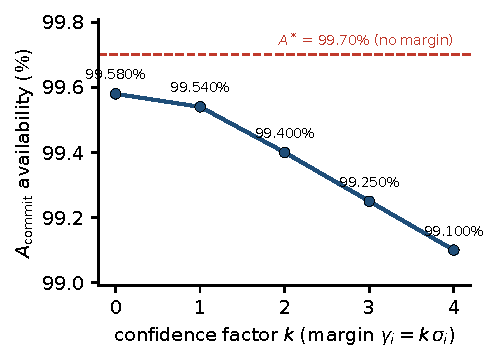
\includegraphics[width=0.72\linewidth]{figures/gamma_sensitivity.pdf}
\caption{Safely-committable envelope $A_{\mathrm{commit}}$ versus the confidence factor $k$ on the running case. $k=0$ recovers the tier-floored envelope; larger $k$ trades commitment aggressiveness for protection. $A^*$ is the theoretical maximum without margin.}
\label{fig:gamma}
\end{figure}

\subsection{Descending Decomposition}\label{sec:thresholds}
The descending pass translates the architect's target $T$ into per-component requirements: \textit{does each CSP's Sub-SLO cover its share of $T$?} Apportioning $T$ uniformly across components treats architecturally heterogeneous services as equal consumers of the global budget---an assumption that fails when, e.g., a storage backend structurally dominates cost relative to a stateless authentication service. We instead weight each component by its structural centrality in $G$:
\[
  w_i = \frac{1 + \deg^-(i)}{\sum_{j \in V}\bigl(1 + \deg^-(j)\bigr)}
\]
The threshold for cumulative metrics is $s_i = w_i \cdot T$; for availability the error budget is distributed as $s_i = 100 - w_i(100-T)$. On the running case ($\deg^-$: UI$\,{=}\,0$, Auth$\,{=}\,$Stor$\,{=}\,1$) a cost target $T=23$\,EUR/h yields $s_{\mathrm{UI}}=4.6$ and $s_{\mathrm{Auth}}=s_{\mathrm{Stor}}=9.2$\,EUR/h, against a uniform $7.7$ for all three---a differentiation that closes the detection gap measured in Section~\ref{sec:eval}. A Sub-SLO $v_i$ short of $s_i$ raises a \emph{descending over-commitment fault}.

\textbf{Complexity.} Each pass traverses the topological order once, propagating a constant number of scalars per edge, so the whole verdict costs $O(|V|+|E|)$ time and $O(|V|)$ space---without ever enumerating the potentially exponential set of root-to-leaf paths. The real 38-service graph below is validated in a few milliseconds; the 200-topology population study of Section~\ref{sec:realistic} runs end-to-end in ${\approx}2.4$\,s ($\approx 12$\,ms per scenario). Analysis cost is dominated by observability data collection.

\subsection{Sustainability under Reconfiguration}\label{sec:translation}
Static validation is insufficient if elasticity rules cannot sustain the SLO: SLOs are functional metrics (e.g., throughput) while triggers are operational parameters (e.g., CPU). A knowledge base of rules $(\mathit{metric}, \mathit{component\text{-}class}) \mapsto (\mathit{operational\ parameter}, \mathit{threshold})$ bridges the gap---e.g.\ sustaining a message broker's throughput SLO requires scaling out before CPU exceeds $80\%$. If the strategy's scale-out transition is guarded by \texttt{cpu\_util > 90\%}, the trigger fires \emph{after} the protective bound is breached and the SLO is violated in $[80\%, 90\%]$: a \emph{reconfiguration fault}. Scale-\emph{in} transitions releasing capacity above the bound are flagged symmetrically. Static envelope validation without an operational model---the prior practice---cannot represent this fault class at all.

%==============================================================================
\section{\texttt{slacheck} in Production: Live Datadog Topology to SLA Verdict}\label{sec:tool}
%==============================================================================

We implemented the methodology in \texttt{slacheck}, a lightweight Python tool. It accepts a hand-written YAML topology (typed edges, Sub-SLAs, margins, reconfiguration state machines) but, critically for practice, can also construct the dependency graph \emph{automatically from a live observability backend}: it discovers the typed topology from Datadog's distributed-tracing service map, enriches each node with per-service trace latencies, extracts the critical path under the user's constraint, computes envelope, weights, and thresholds, and publishes the verdict---achievable envelope, per-service panels along the critical path, and the detected over-commitment faults---as a Datadog dashboard.

We exercised this loop end-to-end on the \emph{train-ticket} benchmark (38 services) deployed on a shared Kubernetes cluster monitored by the Datadog organization of Devoteam's observability practice: live topology discovery from the service map, live trace latencies, envelope computation over the typed DAG, and dashboard publication to the organization's account. The exported dashboard ships with the artifact (Section~\ref{sec:concl}), so the live verdict is inspectable without credentials. On the running case, the tool showed that three conjunctive $99.9\%$ components cap global availability at $99.7\%$ before any margin: the architect's $99.999\%$ goal was structurally impossible and flagged as an ascending fault, giving the engineering team concrete evidence that a topology change (redundant disjunctive providers) was needed \emph{before} signing.

Running against a real backend taught us lessons that the methodology alone does not surface:
\begin{itemize}
  \item[\textbf{L1}] \textbf{Trace sampling starves latency SLOs.} The APM agent's default head-based sampling left only a handful of aggregated latency points per service under moderate load. Sustained load generation plus forcing the tracer sample rate were required before per-service p99 became usable.
  \item[\textbf{L2}] \textbf{Infrastructure proxies are enough for a verdict.} Contractual SLOs are rarely exposed by the backend. A cost estimate from reserved CPU/memory ($\mathrm{cost} \approx \mathrm{cpu\_cores}\cdot p_{\mathrm{cpu}} + \mathrm{mem\_gb}\cdot p_{\mathrm{mem}}$) and an availability proxy from deployment readiness (ready/desired replicas) supported the pre-deployment verdict---reported explicitly as estimates, not billed cost or contractual uptime.
  \item[\textbf{L3}] \textbf{Keep a declared topology beside the live one.} APM records only edges exercised during the observation window. We use the live service map as \emph{provenance} that discovery works, and the documented call graph as a \emph{declared} topology for deterministic, reproducible evaluation; the principal live edges agree with the declared graph.
  \item[\textbf{L4}] \textbf{Filter before you aggregate.} A real organization's service map is far larger than the application under study (${\approx}215$ services in ours); prefix-based service filtering is indispensable, as is reducing the observed cycles (e.g.\ seat\,$\leftrightarrow$\,travel) to a DAG by dropping back-edges.
\end{itemize}

%==============================================================================
\section{Evaluation}\label{sec:eval}
%==============================================================================

\subsection{Mechanism Validation on a Constructed Dataset}\label{sec:eval-dataset}

We first evaluate fault detection on a constructed dataset of 113 injected inconsistencies in three categories: Global-SLO, Sub-SLO, and reconfiguration faults. As Table~\ref{tab:eval} shows, the full method detects all 113. The ablated baseline (series aggregation, uniform decomposition, no reconfiguration model---the closest prior practice) detects 67: it matches on Global-SLO faults, misses 3 of 60 Sub-SLO faults, and all 43 reconfiguration faults. The three Sub-SLO misses arise precisely from uniform decomposition under-allocating to low-centrality components; the structural weights $w_i$ tighten exactly those thresholds and recover all three ($57/60 \rightarrow 60/60$). The reconfiguration column measures \emph{feature coverage}---a fault class prior practice cannot represent---rather than discrimination within a shared capability; the substantive ablated comparison is the Sub-SLO gap. As the dataset is constructed to exercise these mechanisms, the result reads as evidence that each mechanism closes the gap it targets, not as an empirical detection rate over arbitrary architectures.

\begin{table}[htbp]
\caption{Fault detection across scenario categories: ablated baseline vs.\ full method.}
\begin{center}
\begin{tabular}{|l|c|c|c|}
\hline
\textbf{Scenario Category} & \textbf{Injected} &
\textbf{Baseline} & \textbf{Full} \\
\hline
Global-SLO Inconsistencies      & 10 & 10 & 10 \\
Sub-SLO Inconsistencies         & 60 & 57 & 60 \\
Reconfiguration Inconsistencies & 43 &  0 & 43 \\
\hline
\textbf{Total}                  & \textbf{113} & \textbf{67} & \textbf{113} \\
\hline
\end{tabular}
\label{tab:eval}
\end{center}
\end{table}

\subsection{Real-World Systems}\label{sec:casestudy}

We then apply \texttt{slacheck} to \emph{train-ticket} (38 services, 85 documented dependencies; topology discovered live, encoded as a declared graph for reproducibility, cycles reduced to a DAG). The in-degree weights on this real graph are markedly non-uniform---\texttt{ts-order-service} ($w \approx 0.082$), \texttt{ts-station-service} ($0.074$), \texttt{ts-route-service}/\texttt{ts-travel-service} ($0.066$)---so the structural weighting produces a meaningful centrality profile on a real architecture. Under a $99.9\%$ availability target (Table~\ref{tab:casestudy}), the full method aggregates the whole DAG to a $98.36\%$ envelope and raises 6 faults; the critical-path baseline reports an over-optimistic $99.40\%$ and raises 3. The three recovered faults---\texttt{order}, \texttt{station}, \texttt{train}---are high-centrality services that sit \emph{off} the baseline's single path (Figure~\ref{fig:traindag}). The latency target is starker: at $30$\,ms the baseline declares the system \emph{feasible} ($24$\,ms on its path) while the full method raises a fault ($48$\,ms over the full DAG)---a concrete false-negative prevented on a real system. Note the miss here stems from the series critical-path reduction, whereas the dataset above isolates uniform-vs-weighted decomposition: the two evaluations exercise distinct mechanisms.

To confirm the effect is not system-specific, we encode \emph{Online Boutique}, Google's reference microservices demo~\cite{googleboutique}, whose 10-service call graph is extracted from the \texttt{*\_SERVICE\_ADDR} variables of the official manifest (no edges guessed). Under the same $99.9\%$ target the full method aggregates all ten services to a $98.50\%$ envelope while the critical-path baseline again hides the over-commitment. We deliberately encode only systems whose call graph is recoverable from an authoritative manifest.

\begin{table}[htbp]
\caption{train-ticket case study: detection on a real 38-service topology (declared graph, trace-derived metrics).}
\begin{center}
\begin{tabular}{|l|c|c|}
\hline
\textbf{Validation} & \textbf{Baseline (crit.\ path)} & \textbf{Full (typed DAG)} \\
\hline
Achievable availability         & 99.40\% & 98.36\% \\
Faults at avail.\ $\geq 99.9\%$  & 3       & 6 \\
Achievable latency              & 24\,ms  & 48\,ms \\
Verdict at lat.\ $\leq 30$\,ms   & feasible & fault \\
\hline
\end{tabular}
\label{tab:casestudy}
\end{center}
\end{table}

\begin{figure}[htbp]
\centering
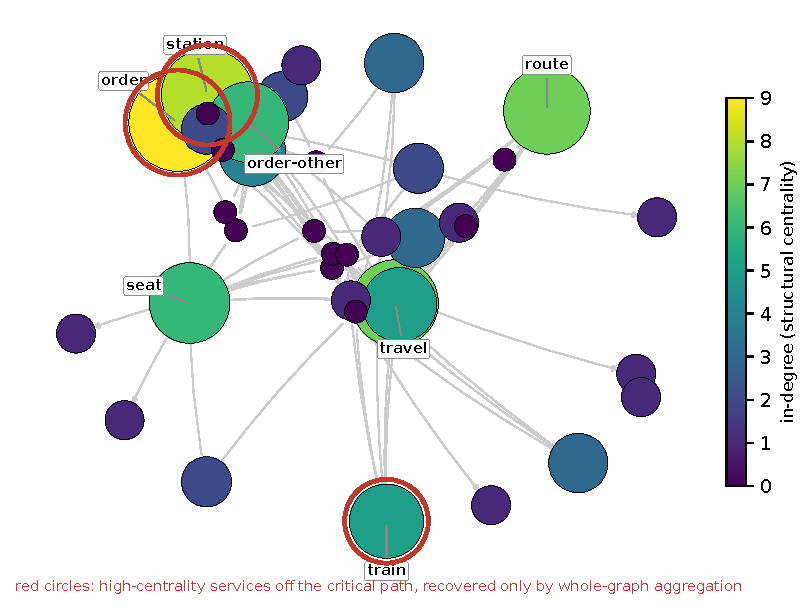
\includegraphics[width=\linewidth]{figures/train_ticket_dag.pdf}
\caption{The \emph{train-ticket} dependency graph (38 services, automatically discovered). Node size and colour encode in-degree. Circled in red: the three high-centrality services that sit off the single critical path a series reduction inspects, recovered as faults only by whole-graph aggregation.}
\label{fig:traindag}
\end{figure}

\subsection{Statistical Validation on a Realistic Population}\label{sec:realistic}

Two real systems show the effect concretely but cannot quantify how often it occurs. We generate 200 synthetic topologies whose \emph{structure} follows distributions reported for production microservice traces at Alibaba~\cite{luo2021alibaba} (heavy-tailed service count, in-degree dominated by one, varying depth), each with one injected Sub-SLO over-commitment on a low-centrality service, placed inside the \emph{discriminating window} $[s^{\mathrm{weighted}}_i, s^{\mathrm{uniform}}_i]$ between the two methods' thresholds. Weighted decomposition detects $89.5\%$ (95\% Wilson CI $[84.5, 93.0]$) against $4.0\%$ ($[2.0, 7.7]$) for uniform (Table~\ref{tab:realistic})---non-overlapping intervals, stable as the population grows.

Because the headline injects faults inside the window, one might suspect the separation is constructed. Two checks say otherwise. First, sweeping the fault cost \emph{through} both thresholds (Figure~\ref{fig:sweep}) shows a genuine threshold effect: below the stricter weighted threshold neither method fires (correctly---no over-commitment exists); past it the weighted method fires immediately, while uniform stays at the floor until the fault outgrows its looser threshold. Uniform decomposition simply tolerates a larger over-commitment before reacting; the headline is one slice of this curve. Second, drawing the injected cost from a log-normal perturbation \emph{independent} of both thresholds (keeping only genuine over-commitments), most faults are large enough for both methods and the gap narrows---but weighted still strictly dominates at $100\%$ ($[98.1, 100]$) versus $89.0\%$ ($[83.9, 92.6]$), because its threshold is never looser. The window figure measures \emph{which method is correct} in the discriminating regime; the independent draw measures \emph{how often it matters} on an unconstructed distribution.

\begin{table}[htbp]
\caption{Statistical validation on a realistic population of 200 Sub-SLO scenarios (Alibaba-like topologies, fixed seed).}
\begin{center}
\begin{tabular}{|l|c|c|}
\hline
\textbf{Decomposition} & \textbf{Detection rate} & \textbf{95\% CI} \\
\hline
Uniform (ablated)  & 4.0\%  & [2.0, 7.7] \\
Weighted (full)    & 89.5\% & [84.5, 93.0] \\
\hline
\end{tabular}
\label{tab:realistic}
\end{center}
\end{table}

\begin{figure}[htbp]
\centering
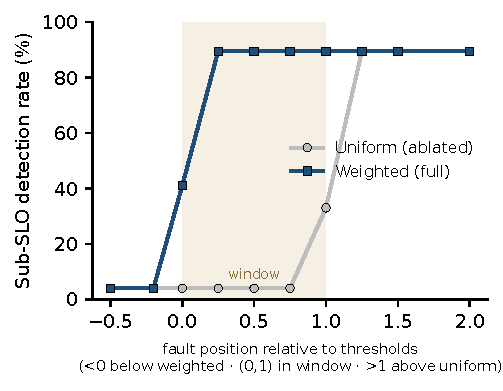
\includegraphics[width=0.9\linewidth]{figures/detection_sweep.pdf}
\caption{Detection as the injected fault moves through both decomposition thresholds (window shaded). Weighted decomposition reacts as soon as the fault exceeds the structurally-correct threshold; uniform tolerates a larger over-commitment. The headline figure is the slice inside the window.}
\label{fig:sweep}
\end{figure}

%==============================================================================
\section{Threats to Validity and Conclusion}\label{sec:concl}
%==============================================================================

\textbf{Threats.} Reconfiguration-fault accuracy is bounded by the expert-curated knowledge base mapping functional SLOs to operational metrics; a flawed mapping yields false verdicts. The margin $\gamma_i$ introduces a manual calibration: $k$ and the estimation window for $\sigma_i$ trade violation probability against commercial competitiveness, with no universal setting---and the tier floor relies on an external infrastructure classification~\cite{turner2006tier} whose mapping to delivered cloud availability we do not validate. On the evaluation: neither the constructed dataset nor the headline population is sampled from production incidents; both quantify \emph{which} method catches a fault when one exists, not how frequently such faults arise. We mitigate this with the position sweep, the independent-distribution draw, two real independently-specified systems, and by grounding the population's structure in published production-trace distributions~\cite{luo2021alibaba}. Finally, when trace-level metrics are unavailable the availability values are readiness or request-success \emph{proxies}, not contractual uptime; live per-service latencies were noisy under the shared cluster's load, so the reproducible case-study figures come from the deterministic declared-topology configuration, with the live run establishing that the pipeline operates end-to-end on real Datadog data.

\textbf{Conclusion.} We presented a pre-deployment validation methodology that computes the safely committable SLA envelope of a multi-cloud composition over a typed dependency DAG, decomposes targets by structural centrality, and validates elasticity rules by operational translation---giving architects a structured answer to \emph{what SLA they can safely commit to}, and preventing a class of violations by construction rather than mitigating them at runtime. The framework is defined per metric by its aggregation operator, so it extends to any SLO whose composition is expressible as one (throughput, durability, RPO/RTO). Future work targets workload-aware structural weights, validation over a corpus of production topologies, and continuous runtime conformance checking.

\textbf{Artifact availability.} The \texttt{slacheck} tool, evaluation scripts, fault-injection and topology generators (fixed seeds), both real-system topologies, and the exported live dashboard are publicly available and reproduce every number and figure offline, without credentials.\footnote{\url{https://github.com/Wassbdr/slacheck}} % TODO(wassim): créer le repo public (branche squashée sans PII) et confirmer l'URL avant soumission.

%==============================================================================
% References
%==============================================================================
\bibliographystyle{IEEEtran}
\bibliography{refs}

\end{document}
